\chapter{Оптимизация параметров}\label{optimization}
Код FAINA позволяет не только расчитывать излучение заданных источников, но и фитировать наблюдательные данные модельными, подбирая необходимые параметры. Реализованы методы оптимизации, пригодные для произвольного числа параметров и широкого класса моделей источников. В качестве целевой функции используется взвешенная сумма квадратов отклонений по всем наблюдательным точкам $f = \sum \frac{(F_i - F_{obs,i})^2}{\sigma_i^2}$, где $F_i$ - расчетная спектральная плотность потока излучения, $F_{obs,i}$ - наблюдаемая спектральная плотность потока излучения, $\sigma_i$ - её погрешность. 

Реализованные методы оптимизации делятся на два типа - те, которые рассматривают излучение в один момент времени, либо постоянные во времени, и те, которые учитывают эволюцию источников и используют наблюдения в разные моменты времени. В последнем случае пользователю необходимо самостоятельно указывать, как меняются параметры источника со временем, см. \ref{timeDependentSource}.

\subsection{Фитирование источников, не зависящих от времени}
\begin{figure}
	\centering
	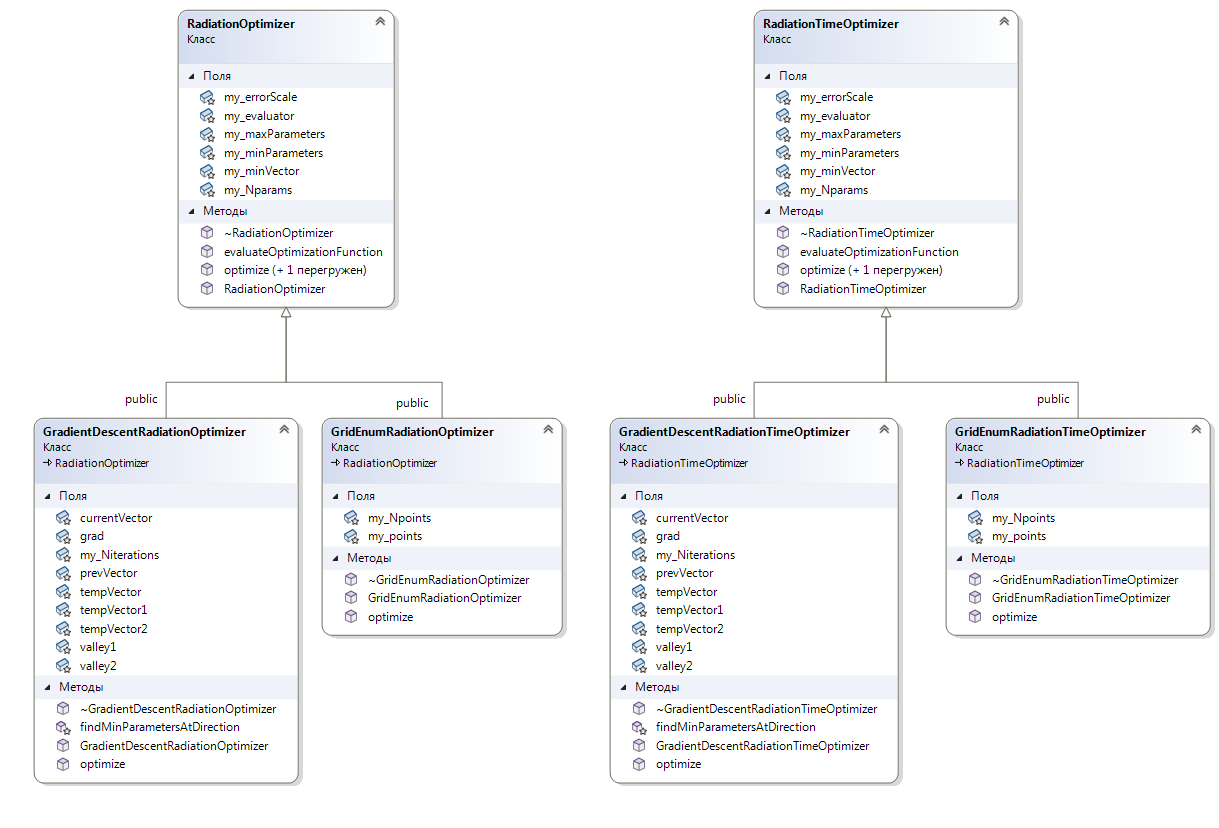
\includegraphics[width=10.5 cm]{./fig/radiationOptimizer.png} 
	\caption{Схема наследования классов оптимизаторов}
	\label{radiationOptimizer}
\end{figure}
\subsection{Фитирование источников, зависящих от времени}
\begin{figure}
	\centering
	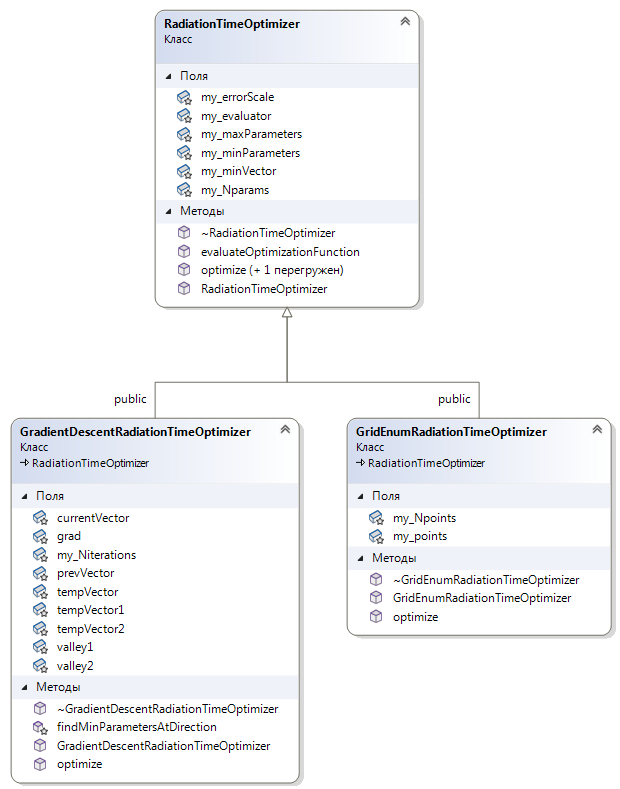
\includegraphics[width=10.5 cm]{./fig/radiationOptimizerTime.png} 
	\caption{Схема наследования классов оптимизаторов, зависящих от времени}
	\label{radiationOptimizer}
\end{figure}